% !TEX TS-program = xelatex
%
% Created by Chris on 2020-07-19.
% Copyright (c) Chris von Csefalvay, 2020.
\documentclass{article}
\usepackage{amsmath}
\usepackage{polyglossia}
\usepackage{hyperref}

% Bibliography styling
\usepackage[super,square,sort&compress,numbers]{natbib}
\bibliographystyle{unsrtnat}
\usepackage{url}
\urlstyle{same}

% Language and hyphenation
% \usepackage[english]{babel}
\usepackage[htt]{hyphenat}

% Graphics
\usepackage{graphicx}

\hypersetup
{
  pdftitle   = {A differential game analysis of social distancing in COVID-19},
  pdfauthor  = {Chris von Csefalvay}
}

\title{A differential game analysis of social distancing in COVID-19}
\author{Chris von Csefalvay}

\begin{document}

\maketitle

\begin{abstract}
    Abstract
\end{abstract}

\section{Introduction} % (fold)
\label{sec:introduction}
Where an infectious disease is not amenable to population-level prevention through vaccination and risks are non-trivial, non-pharmaceutical interventions (NPIs) remain the principal tool of public health to respond to an outbreak. This is the case with novel infectious diseases that have no specific treatment and no prophylactic (vaccine) available. In the absence of pharmaceutical interventions of proven effectiveness, in particular prophylactically, the main public health response to the emerging pandemic of COVID-19, a viral syndrome caused by the (+)ssRNA virus SARS-CoV-2 (order \emph{Nidovirales}, family \emph{Coronaviridae}, genus \emph{Betacoronavirus}, subgenus \emph{Sarbecovirus}), has rested principally on NPIs, first and foremost social distancing and ancillary steps intended to facilitate that.

In general, any course of conduct that reduces the encounter rate between an individual and other individuals can be considered a form of social distancing. This may be brought about through limiting public facilities for such encounters ('lockdowns'), through limiting individual gatherings by size ('large-gathering bans') and through encouraging individual social distancing. From the perspective of game theory, social distancing can be viewed as a non-cooperative game of a population $P_{1 \ldot n}$ of size $n$, where at any given time $t \in [t_0, t_{e}]$, the strategy adopted by $p_i$ is denoted as $\sigma (p_i, t)$. For the sake of simplicity, we assume that distancing is either not exercised at all or perfectly exercised, i.e. $\sigma (p_i, t) \in \{ 0, 1 \}$. Then, for the entire population, the overall strategy can be described as 

\begin{equation}
	\bar{\sigma}(P, t) = \frac{\displaystyle \sum_{i = 0}^n \sigma(p_i, t)}{n}
	\label{eq:overall_strategy}
\end{equation}

\noindent and for the entire time period, from $t_0$ to the endpoint $t_e$ (which may be eradication, elimination, natural extinction of the pathogen, the availability of a vaccine or a combination thereof), for discrete time $t$,

\begin{equation}
	\bar{\bar{\sigma}}(P) = \frac{\displaystyle \sum_{i = 0}^n \displaystyle \sum_{j = 0}^{t_e - t_0} \sigma(p_i, j)}{n (t_e - t_0)}
	\label{eq:overall_strategy_over_time}
\end{equation}

However, with each course of conduct, there is associated a cost $J(\sigma)$. For simplicity's sake, let us consider these costs to be governed by the following three precepts.

\begin{enumerate}
	\item A person $p_i \in P$ opting for strategy $1$ (social distancing) will incur $c_d$, the immediate costs of distancing. These may be social (lessened social interaction), psychological (lessened access to support systems), economic (lower access to facilities to earn) or simple matters of convenience (access to amenities). While $c_d$ is somewhat dependent on $\bar{\bar{(P)}}$ (thus not distancing does not yield a benefit to a lone social distancer in terms of access to amenities if all of the latter are closed), it can be assumed to be largely constant.
	\item A person $p_i \in P$ opting for strategy $1$ will gain a benefit of $b_d$, which represents an individual's reduced risk of illness due to their own distancing from possibly infected persons.
	\item Regardless of their individual strategy, a person $p_i \in P$ will gain a benefit $b_s$ that is very closely approximated by a function of the overall strategy adopted by society, so that $b_s(p_i, t) = f(\bar{\sigma}(P, t))$ for $p_i \in P$.
\end{enumerate}

Then, assigning the variable $c_s$ to represent the cost of illness (economic loss, medical costs, long-term health risks), we can express the cost functions of each strategy, $\sigma_1$ (social distancing) and $\sigma_0$ (no social distancing), as

\begin{equation}
	J_{\sigma_1}(p_i, t) = c_d - b_d r_d c_s - f(\bar{\sigma}(\delta_P, t))
\end{equation}

\noindent and

\begin{equation}
	J_{\sigma_0}(p_i, t) = r_d c_s - f(\bar{\sigma}(\delta_P, t))
\end{equation}

\noindent for $p_i \in P$, where $r_d$ denotes $p$'s level of risk and $\delta_P$ denotes the proportion of individuals that adopt $\sigma_1$. And consequently, it holds for the. population level cost $\bar{J}$ that

\begin{equation}
	\bar{J}(P, t) = \frac{\delta_P J_{\sigma_1}(P, t) + (1 - \delta_P) J_{\sigma_0}(P, t)}{n}
\end{equation}

As Reluga (2010) notes, the effect of social distancing diminishes with the increase in participants, the phenomenon of diminishing returns.\cite{reluga2010game} Thus, as the number of individuals in $P$ opting for social distancing increases, the marginal increase by another social distancer diminishes. This can be represented by a discount factor $h$, to yield

\begin{equation}
	\bar{J}(P, t) = e^{-ht} \Big( \frac{\delta_P J_{\sigma_1}(P, t) + (1 - \delta_P) J_{\sigma_0}(P, t)}{n} \Big)
\end{equation}

However, because individual decisions affect the overall gain (due to the component dependent on $\bar{\sigma}(P, t)$), our principal concern is not with individual action but with analysis of such strategies on a population level. This paper will in the following conceptualise infectious disease in a population as a differential game over a differential equation form of the compartmental model first described by Kermack and McKendrick\cite{kermack1927contribution} and, since its publication in 1927, widely adapted and adopted.\cite{vstvepan2007kermack,roberts1999kermack,capasso1978generalization}

% section introduction (end)

\section{Methods} % (fold)
\label{sec:methods}

Given a population of $n$ under the assumption that reinfection is impossible (as, e.g., in the case of measles) or rare (as is the case for SARS-CoV-2\cite{edridge2020human,deng2020primary,bao2020reinfection}), and neglecting for the time being the vital dynamics (birth, unrelated death, migration) of the population, the dynamics of any population can be modelled as a system of ordinary differential equations

\begin{equation}
	\begin{aligned}
		\frac{dS}{dt} = - \frac{\beta S I}{n} 								\\
		\frac{dI}{dt} = \frac{\beta S I}{n} - \gamma I 						\\
		\frac{dR}{dt} = \gamma I
	\end{aligned}
	\label{eq:sir_equation}
\end{equation}

\noindent under the assumption of $S + I + R = 0$, where $S$ represents susceptible individuals, $I$ represents infected/infectious individuals and $R$ accounts for removed individuals (mortality and recovery to immunity). Even in the absence of firm evidence as to whether SARS-CoV-2 infection followed by recovery would engender lifelong immunity or not,\cite{roy2020covid,ota2020will,lin2020duration} it can be assumed in the short term -- based on evidence from MERS-CoV and SARS-CoV -- that in the short term, survivors remain immune,\cite{prompetchara2020immune} and consequently the number of individuals in $R$ does not decrease.

For a population $P$ of size $n$ that pursues the population-level aggregate of strategies described by $\bar{\sigma(P)}$, the dynamics described above in Equation~\eqref{eq:sir_equation} becomes

\begin{equation}
	\begin{aligned}
		\frac{dS}{dt} = - \bar{\sigma}(P) \frac{\beta S I}{n} 				\\
		\frac{dI}{dt} = \bar{\sigma}(P) \frac{\beta S I}{n} - \gamma I 		\\
		\frac{dR}{dt} = \gamma I
	\end{aligned}
	\label{eq:sir_strat_equation}
\end{equation}

\begin{figure}
	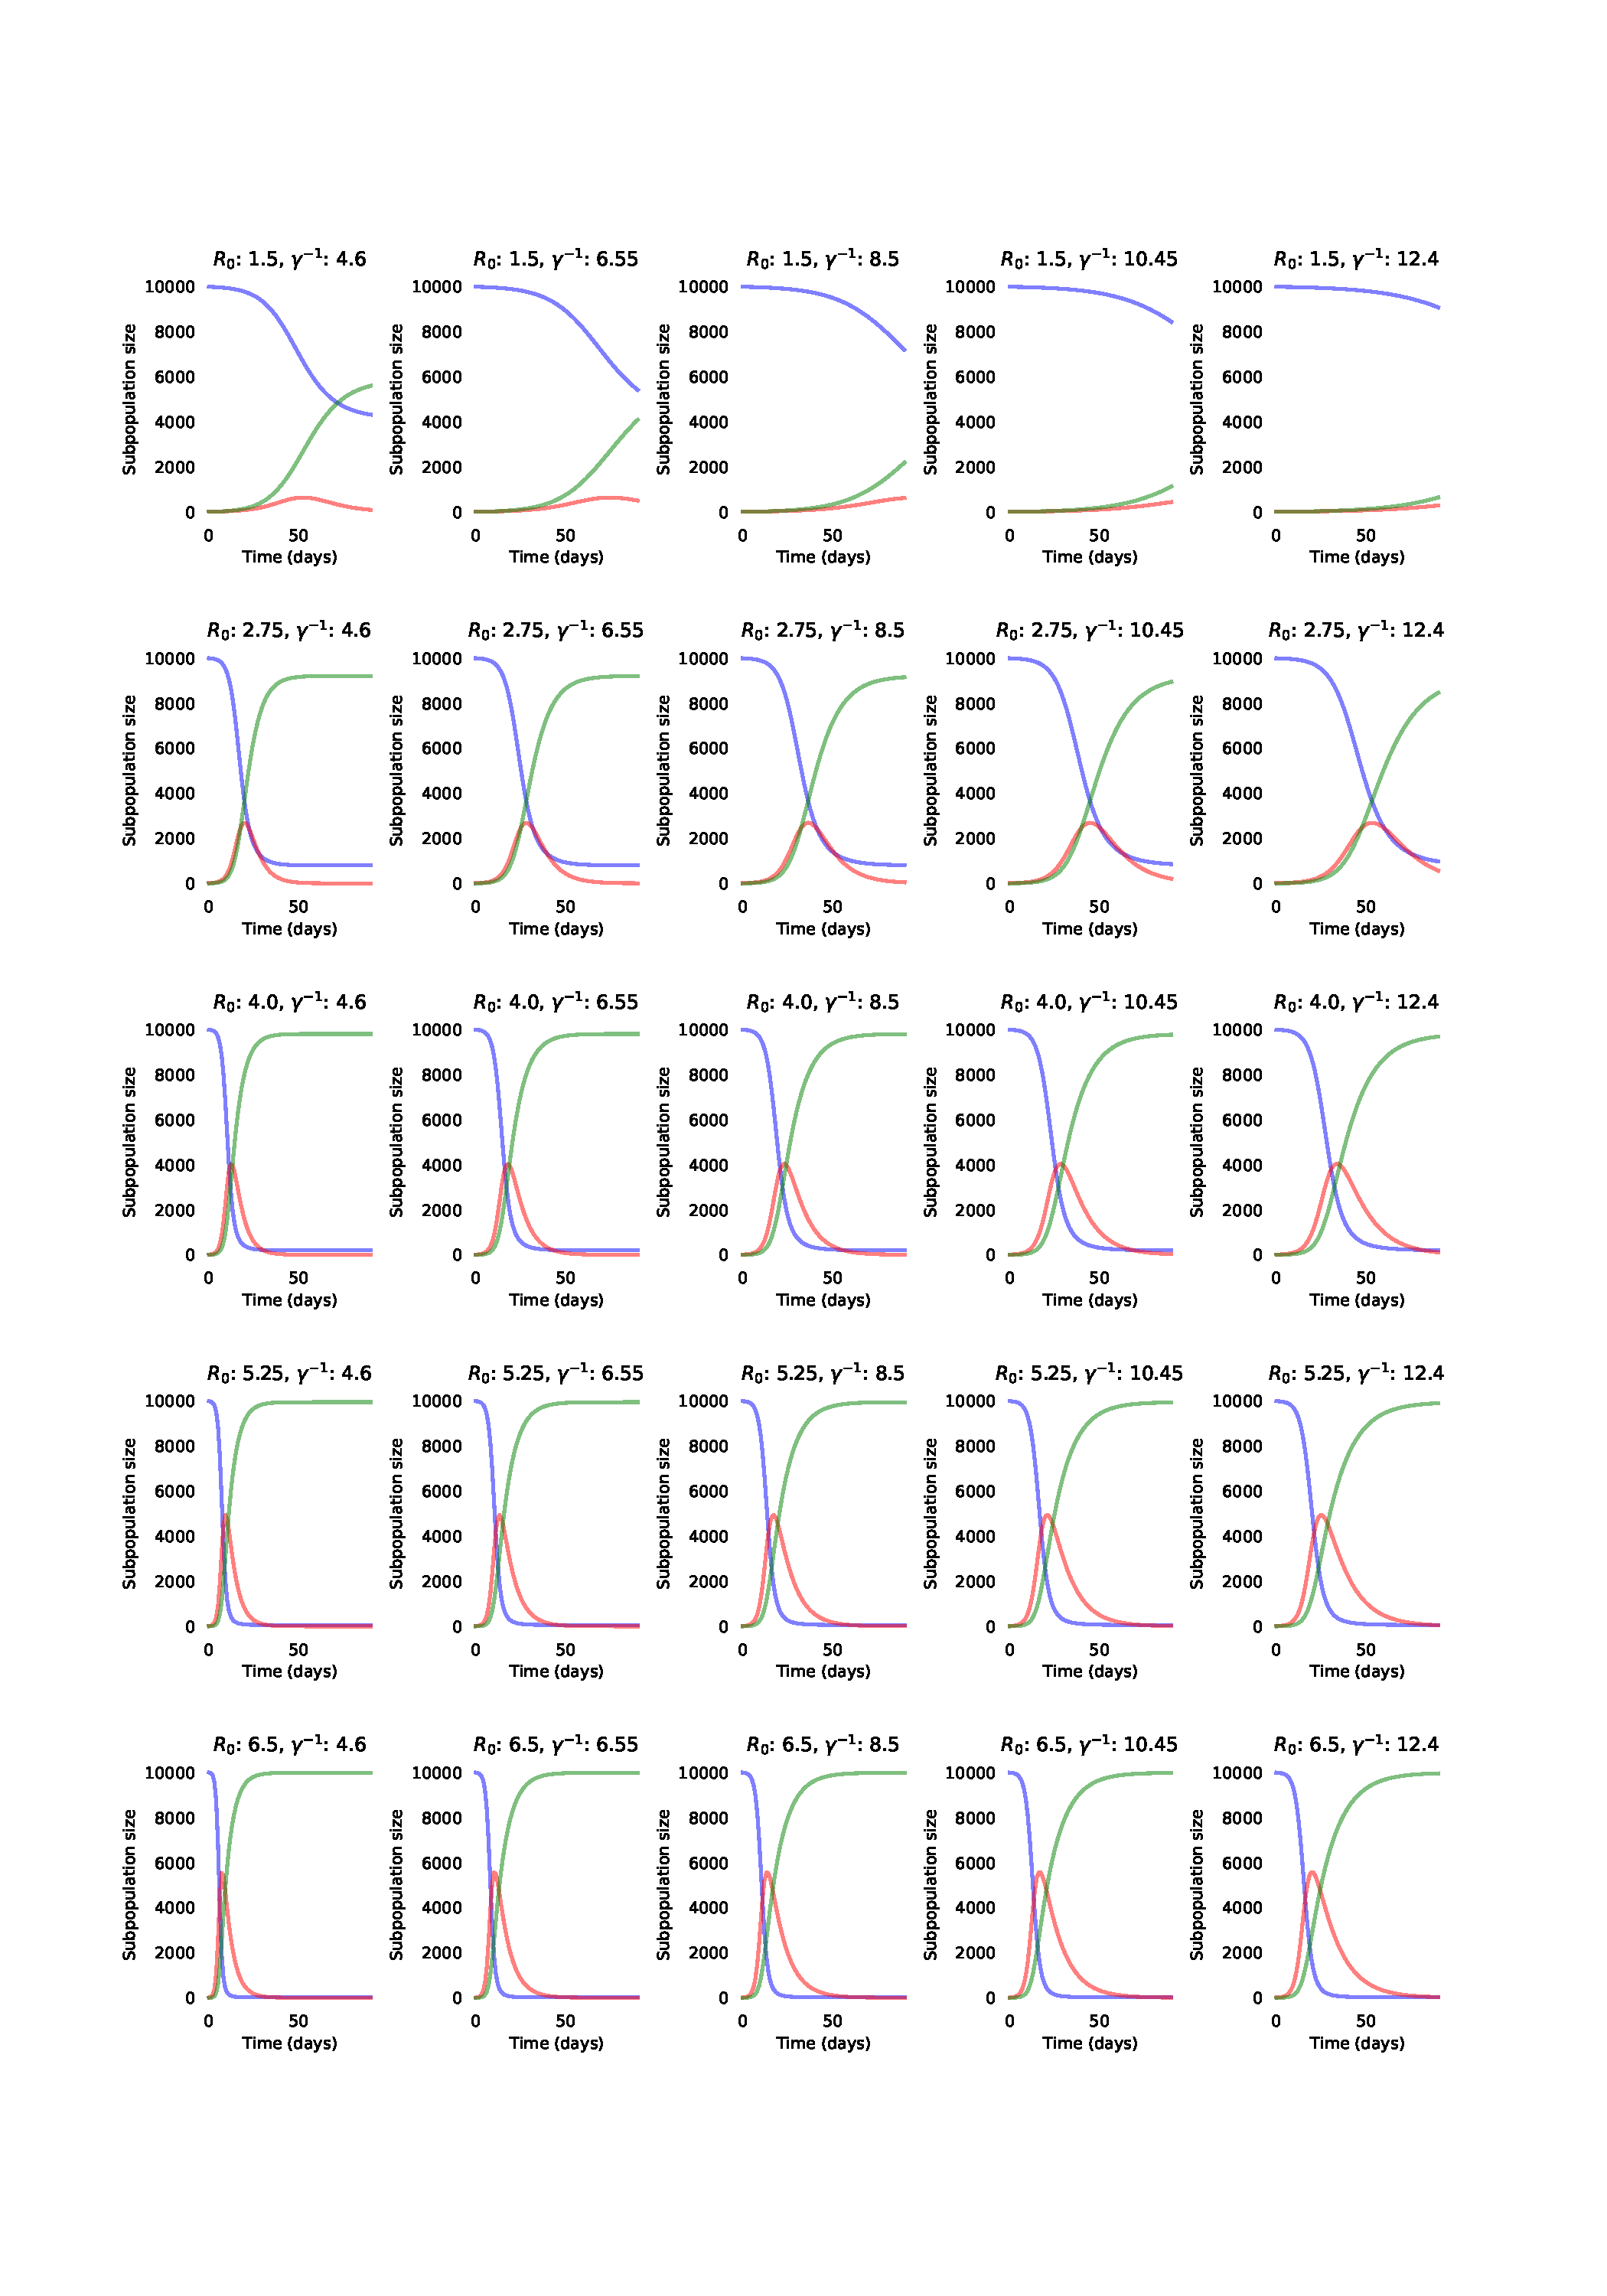
\includegraphics[width=\linewidth]{figures/fig1-odes}
	\caption{Some quantitative solutions for the SIR model's population dynamics over values of $R_0$ between 1.5 and 6.5, and values of $\gamma$ between $1/4.6$ and $1/12.4$ over a base population of 10,000. For each plot, $\beta$ is inferred from an $R_0$ value of 2.67, based on Liu et al. (2020),\cite{liu2020reproductive} and the $\gamma$ parameter. The susceptible population is displayed in blue, while infected/infectious cases are marked in red and recovered cases in green.}
	\label{fig:ode_solutions}
\end{figure}

The fraction $\frac{\beta n}{\gamma}$ equals the basic reproduction number, $R_0$. For SARS-CoV-2, estimates of $R_0$ range from 1.4 to 6.49, with studies that relied on statistical estimation of $R_0$ ranging from 2.20 to 3.58, with an average of 2.67\cite{liu2020reproductive} $\gamma$, on the other hand, can be estimated as the invers of the number of days of illness, which can be approximated as $8.5 \pm 3.9$ days. Figure~\ref{fig:ode_solutions} describes some analytical solutions for the differential equations of Equation~\eqref{eq:sir_equation} over a range of plausible values of $R_0$ and $\gamma$ under the assumption of an $R_0$ of 2.67.

The ODEs of Equation~\eqref{eq:sir_equation} can then be parametrised with the population-level strategy (Equation~\eqref{eq:sir_strat_equation}). 

% section methods (end)

\bibliography{bibliography}

\end{document}
